\begin{figure}
\centering
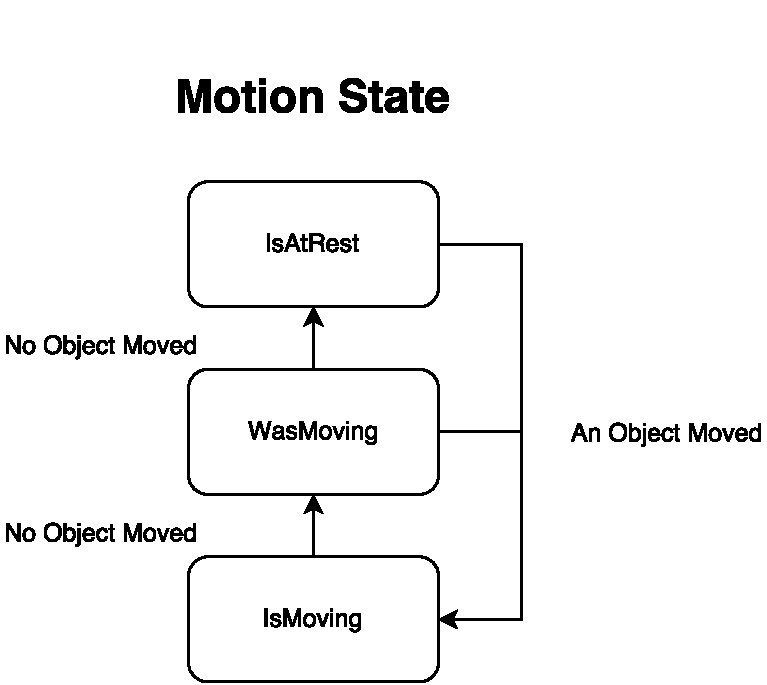
\includegraphics[width=.6\linewidth]{figures/statediagrams/motion-states.pdf}
\caption{motion-states}
\label{fig:motion-states}
\end{figure}

We want to know whether the current path we are following, is still valid or a collision might be occur, should that we can recalculate and plan a new collision free course for the newly changed environment, the state machine depicted in fig.~\ref{fig:motion-states} is responsible for this.

Similarly when a possible target object changes its orientation or location/position in the environment, we would want to recalculate the path and valid grasp or possibly even reconsider which target to pick up. fig.~\ref{fig:motion-states}.

We could do this every frame but as some significant time may be spend calculating such path in a difficult environment, we only want to recalculate when the environment changes.

\begin{figure}
\centering
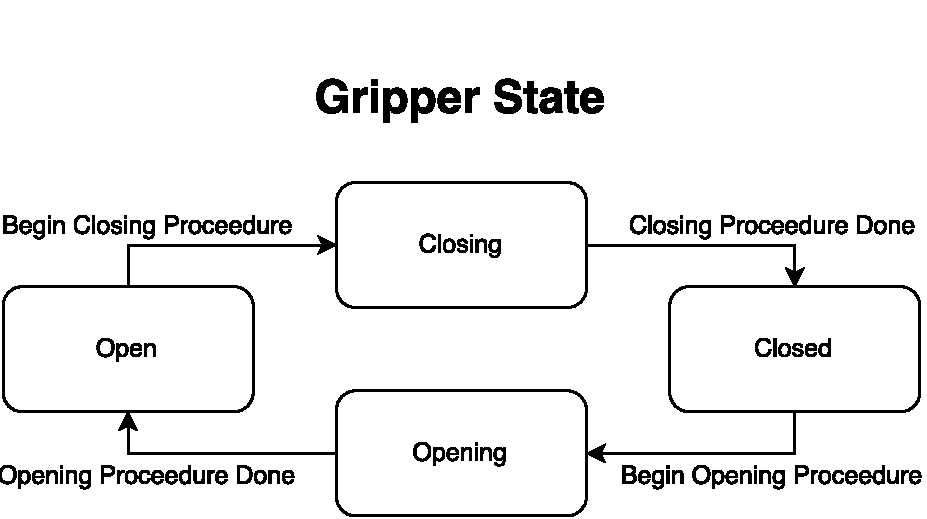
\includegraphics[width=.6\linewidth]{figures/statediagrams/gripper.pdf}
\caption{gripper}
\label{fig:gripper}
\end{figure}

Throughout the simulation we want to track whether the grippers claw is in an open or closed state. Because the simulation runs in discrete time steps means the gripper can be closing to reach a closed state or opening to an open state. Another way to track this was with a percentage but because the closed state position is not a fixed but in fact is dependent on the orientation, position and size of the target object the gripper is picking up, this simpler two static state solution was chosen, depicted in fig.~\ref{fig:gripper}.


\begin{figure}
\centering
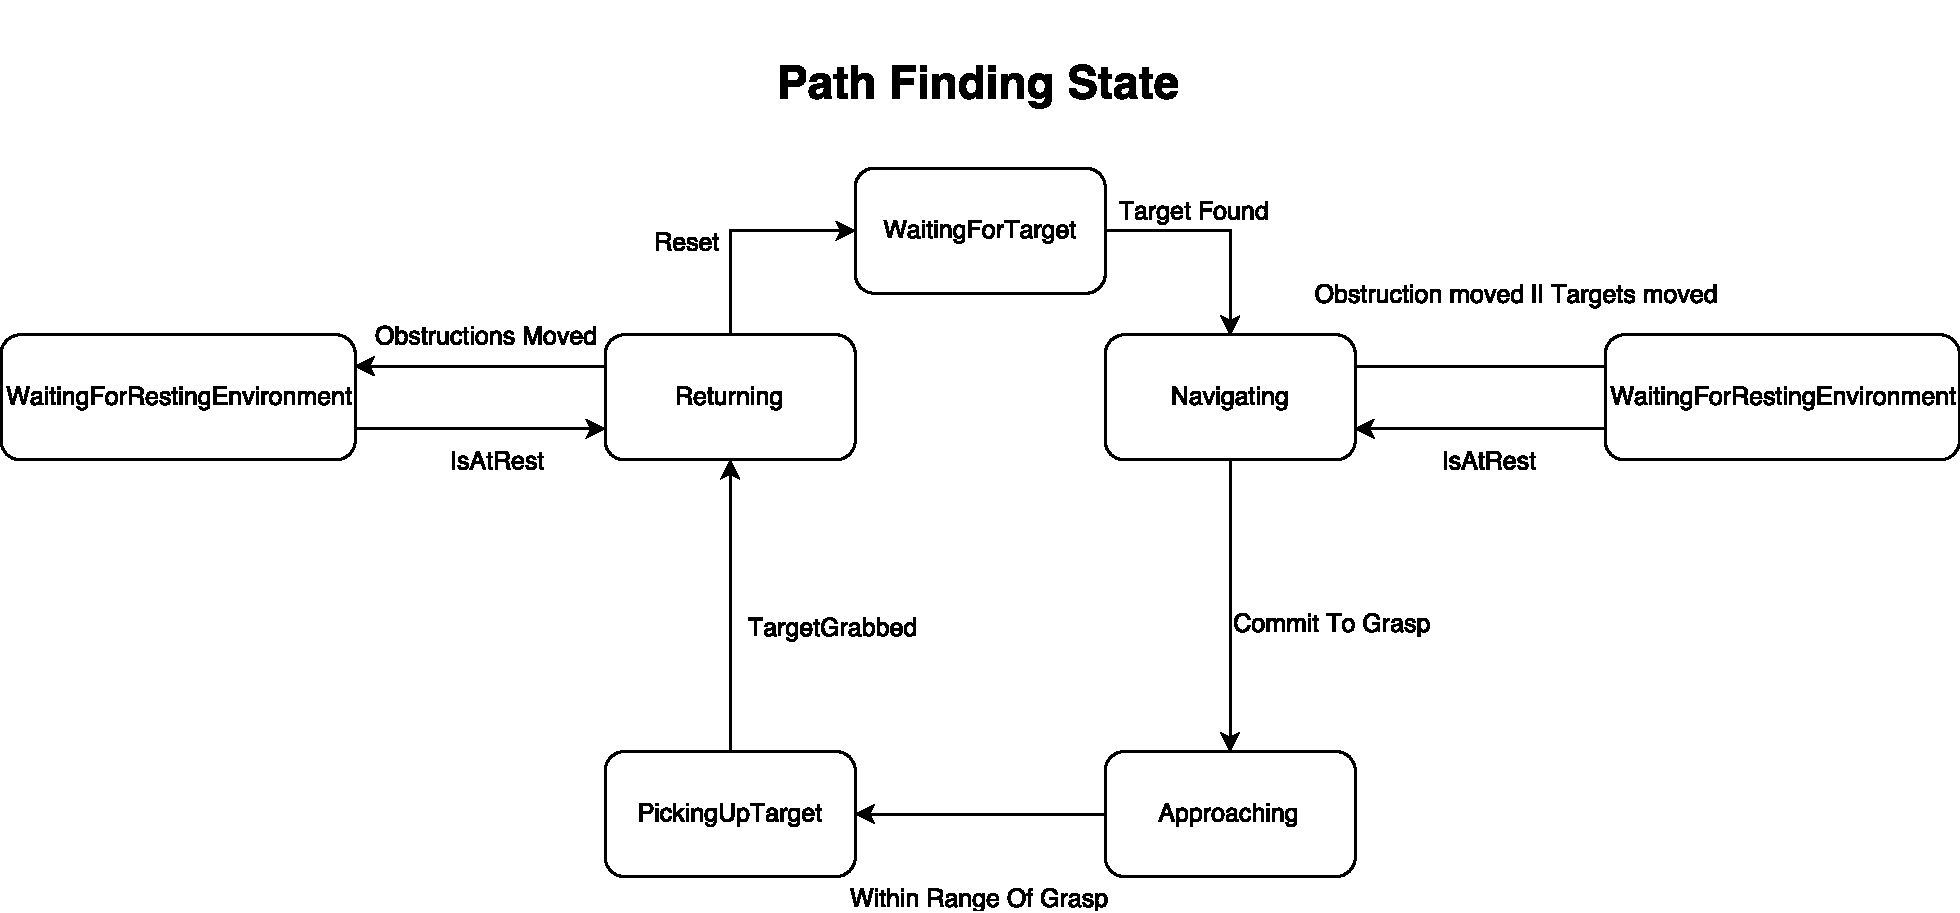
\includegraphics[width=\linewidth]{figures/statediagrams/path.pdf}
\caption{path}
\label{fig:path}
\end{figure}

Along the planned path the gripper is travelling, the gripper transitions through a number of phases that changes its behaviour slightly, like not rotating according to the targets orientation anymore or waiting for the environment to be at rest before continuing. fig.~\ref{fig:path} shows these states or phases if you will.

\begin{figure}
\centering
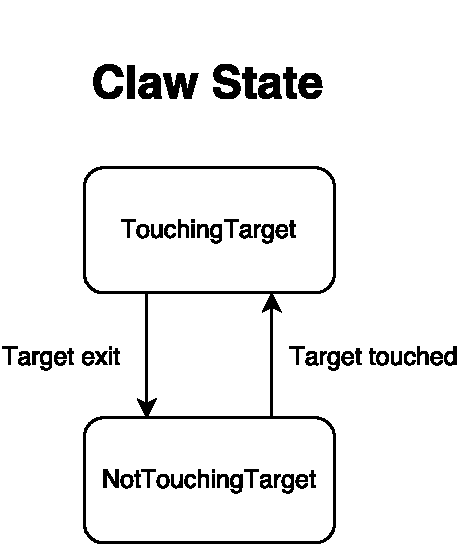
\includegraphics[width=.3\linewidth]{figures/statediagrams/claw-states.pdf}
\caption{claw states}
\label{fig:claw}
\end{figure}

Both claws of the gripper can possibly interacting the target be touching it, thereby also be able to affect its position and orientation. The two states for each claw indicates whether or not we have a secure grasp around the object we are picking up. If the target is only touching one claw it is possible that the object, in this case fish, will just slip out of the gripper during pick up procedure or travel procedure, fig.~\ref{fig:claw} depicts the states for these claws.

\begin{figure}
\centering
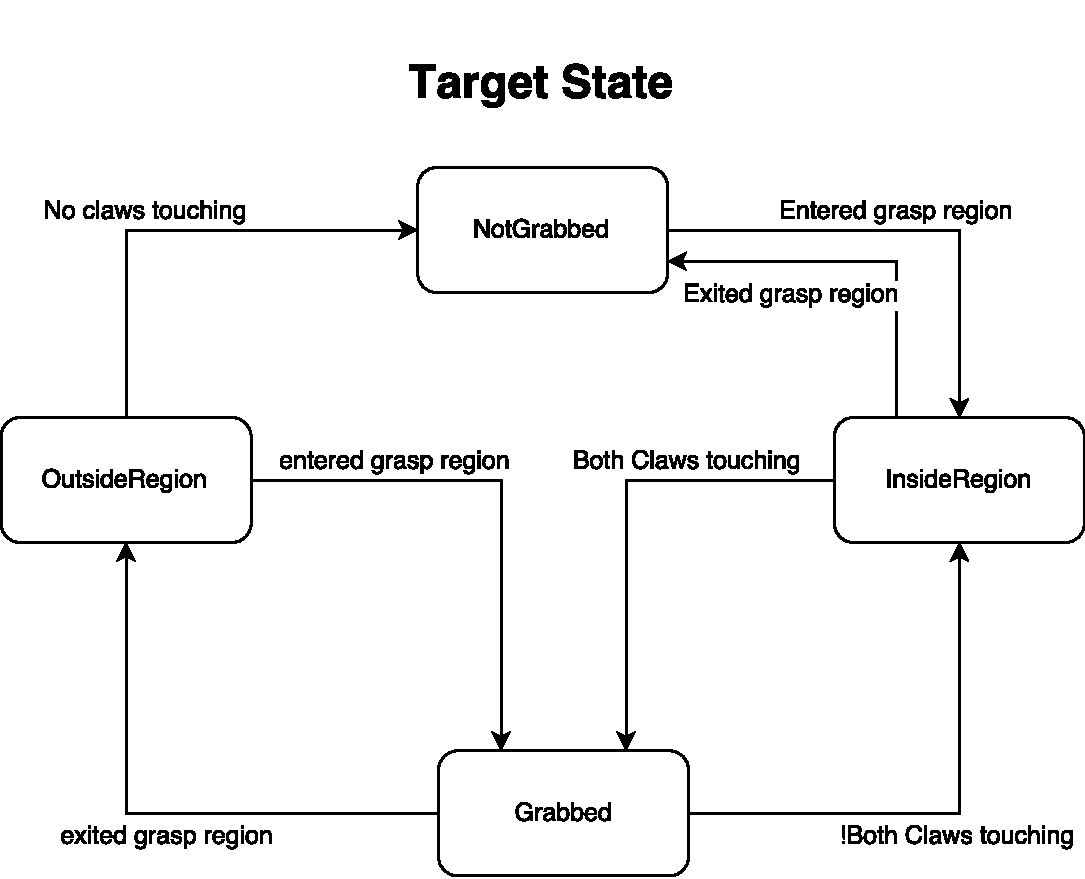
\includegraphics[width=.8\linewidth]{figures/statediagrams/target.pdf}
\caption{target}
\label{fig:target}
\end{figure}

The state machine depicted in fig.~\ref{fig:target}, tries to capture our current belief of the state of the target being picked up, it is possible that we lose the target during travel to destination or that we fail to pick it up in the first place. When picking up the target we are tracking whether the target is inside the region of the gripper where we expect a secure grasp, when this is the case we can procedure on top closing the closing claws and secure the target in place in the gripper.